\documentclass[conference]{IEEEtran}
\IEEEoverridecommandlockouts
% The preceding line is only needed to identify funding in the first footnote. If that is unneeded, please comment it out.
%\usepackage{cite}
\usepackage{amsmath,amssymb,amsfonts}
\usepackage{algorithmic}
\usepackage{graphicx}
\usepackage{subfig}
\usepackage{textcomp}
\usepackage{xcolor}
\def\BibTeX{{\rm B\kern-.05em{\sc i\kern-.025em b}\kern-.08em
    T\kern-.1667em\lower.7ex\hbox{E}\kern-.125emX}}
%% own packages
\usepackage{multirow}
\usepackage{booktabs}
\usepackage[hidelinks]{hyperref}
\usepackage[capitalise]{cleveref}
\usepackage{csquotes}
\usepackage{blindtext}
\usepackage{enumitem}

\usepackage[backend=biber, style=numeric, sorting=none]{biblatex} %Zitate mit BibTeX  %, sorting=none "richtige"
\addbibresource{ML-literature.bib}

% Reihenfolge der Nummern
%, citestyle=alphabetic-verb

\begin{document}

\title{A machine learning approach to predict a vehicles velocity using dashcam video footage}

\author{\IEEEauthorblockN{Florian Wolf}
\IEEEauthorblockA{\textit{Department of Mathematics and Statistics, University Konstanz}\\
Konstanz, Germany\\
florian.2.wolf@uni-konstanz.de}
\and
\IEEEauthorblockN{Franz Herbst}
\IEEEauthorblockA{\textit{Department of Physics, University Konstanz} \\
Konstanz, Germany\\
franz.herbst@uni-konstanz.de}
}

\maketitle

\begin{abstract}
Calculating the velocity of a moving camera relative to its surrounding, the so-called visual odometry 
problem, is a very challenging task and heavily studied in the area of computer vision. Especially
in the field of self-driving cars, a fast and dependable velocity calculation is a high priority.
In this report we will give a machine learning approach to solve the visual odometry problem, using 
optical flow fields combined with convolutional neuronal networks, as well as siamese neuronal networks.
We use a data set with real world dashcam footage and even extend the data by gathering our own
driving videos.
change
\end{abstract}

\begin{IEEEkeywords}
deep learning, computer vision, visual odometry, convolutional neuronal network, siamese network,
optical flow
\end{IEEEkeywords}

\section{Introduction}

Autonomous driving is considered to have a key role in the future of human mobility. Recently the topic has therefore gained great attention in research, economy and politics \cite{Maurer2016}. In this project, we approach this topic in a related, but more simplified setup and present several machine learning techniques and network architectures.

\subsection{Aim of the project}
\label{subsec:AimAndMeasure}

The goal of this project is to predict the velocity of a car based on a dashcam video, inspired by the \emph{comma}\footnote{\url{https://comma.ai/}} speed challenge\footnote{\url{https://github.com/commaai/speedchallenge}} published in 2018. To achieve this goal, we use optical flow analysis to preprocess the data and neuronal networks with different structures (classical and siamese) to predict the velocity. In order to measure the quality of the predictions, we use the mean squared error (MSE) of the measured velocity.

\section{Data collection, analysis and preprocessing}

To start the project we used the database given in the \emph{comma} speed challenge project, which consists of a 17 minute training video (20400 frames) and the corresponding car velocity, as well as a 9 minute test video without labels, to validate the model on an unknown data set.

\subsection{Data collection}

Due to our limited computational power, we mainly used this data set to study different training techniques and model architectures. Still we could not expect good generalization for this rather small pool of training data. We therefore developed a technique to acquire more data that needed minimal resources. We used the open source smartphone apps \emph{open camera} and \emph{open street maps} to cast a video while driving and map the velocity using GPS at the same time. So we were able to train our final model with 1 hour 40 minutes of video data.

\subsection{Data analysis}
\label{subsec:dataAnalysis}

In order to evaluate our raw data with the model, we analysed our dataset concerning the recorded images and driving scenarios. The original frames have a size of $(640,380,3)$ pixels (RGB). To reduce the computation time, we cut the borders of the frames to exclude parts not needed for detection and sampled them down to half of their pixel size.

\begin{figure}[ht]
	\vspace{-0.5cm}
	\centering
	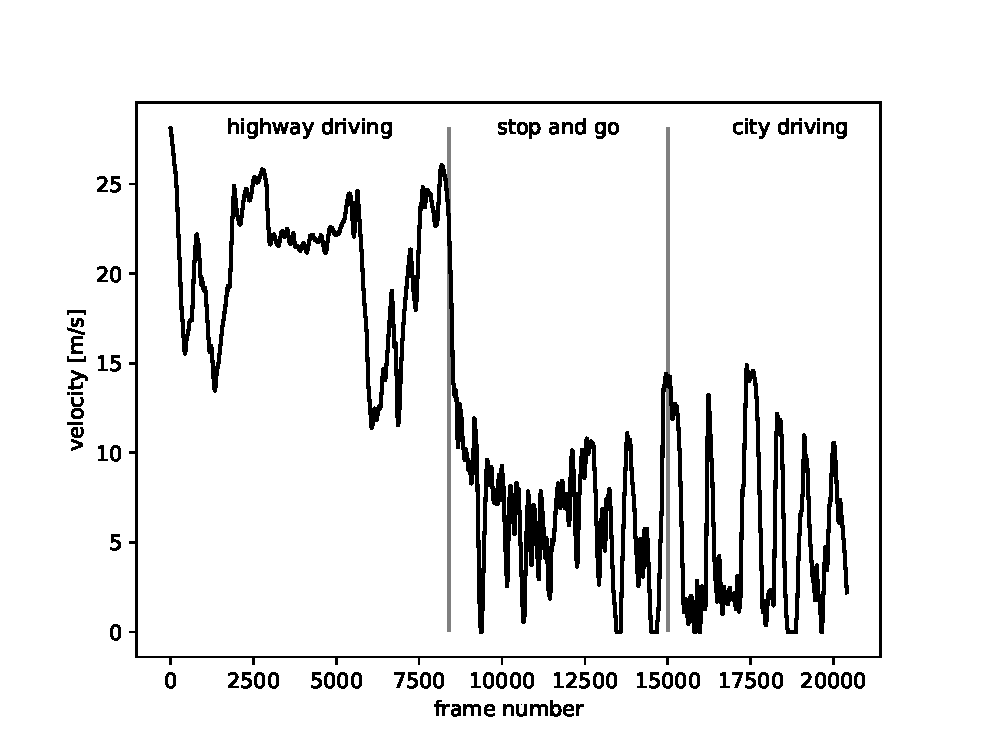
\includegraphics[width=0.7\columnwidth]{./imgs/plot_speed_time_new_splitting.eps}
	\caption{Distribution of the velocities of all frames in the training video, including the three categories.}
	\label{fig:SpeedPerFrameDistributionNewSplitting}
	\vspace{-0.2cm}
\end{figure}

To visualize the training process in different driving scenarios, we plotted the velocity in dependence of the frame number (\cref{fig:SpeedPerFrameDistributionNewSplitting}). After additional evaluation of the video we were able to classify three different driving scenarios: \emph{highway driving} with high and relatively steady velocities, \emph{stop and go} with low and fluctuating velocities, as well as \emph{city driving} with very abrupt speed changes between medium and very low velocities. Every driving scenario is represented with around one third of the training data.

We would then evaluate the predictions of each model $p(x_i)$ to the input data $x_i$ using the mean squared error with respect to the real value of the velocity $y_i$.
\begin{align*}
	\mathcal{L} = \frac{1}{N} \sum_{i=1}^{N} (p(x_i) - y_i)^2
\end{align*}
In order to classify the resulting value, we used the velocity plot and the 
following rough classification\footnote{These rules do only apply on datasets with an equal distribution 
of all driving scenarios}:
\begin{table}[h!]
\normalsize
\centering
\begin{tabular}{r l}
$\sqrt{\mathcal{L}} \gtrsim 16$: & no fitting\\
$16 \gtrsim \sqrt{\mathcal{L}} \gtrsim 10$: & average velocity fitted\\
$10 \gtrsim \sqrt{\mathcal{L}} \gtrsim 5$: & scenarios detected\\
$5 \gtrsim \sqrt{\mathcal{L}} \gtrsim 1$: & variances within scenarios detected\\
$1 \gtrsim \sqrt{\mathcal{L}}$: & perfect fitting
\end{tabular}
\caption{Classification of the result based on the square root of the MSE.}
\end{table}

%\begin{itemize}
%\item $\sqrt{\mathcal{L}} \gtrsim 16$: \textit{no fitting}
%\item $16 \gtrsim \sqrt{\mathcal{L}} \gtrsim 10$: \emph{average velocity fitted}
%\item $10 \gtrsim \sqrt{\mathcal{L}} \gtrsim 5$: \emph{scenarios detected}
%\item $5 \gtrsim \sqrt{\mathcal{L}} \gtrsim 1$: \emph{variances within scenarios detected}
%\item $1 \gtrsim \sqrt{\mathcal{L}}$: \emph{perfect fitting}
%\end{itemize}
For the training process we used a splitting of 80\% training data and 20\% validation data. Initially, 
we choose a hard splitting of the entire data, but this neglects the distribution of different driving 
scenarios in the video. Therefore we went on first splitting the data into the driving scenarios with 
then assigning training data and validation data on each.

\subsection{Preprocessing}

After the previously explained preparation steps, we needed to find a method to extract information 
about the motion of the vehicle, to be able to predict its velocity. There are two ways of doing this: 
either fit two following frames into a network, which will be discussed later, or calculate the relative 
motion between two frames, the so-called \emph{optical flow}, and fit the results into a model.

To calculate the optical flow, we used the \emph{Farneback pyramid method} \cite{Farneback2003}.
The idea of this method can be split up into two main steps: First, use a polynomial expansion of the 
image $f$ and second, solve the optical flow equation
\begin{align*}
\partial_x f \cdot V_x + \partial_y \cdot V_y + \partial_t f = 0
\end{align*}
for different resolutions of the image (pyramid structure). This methods yields a dense optical flow 
field $V$ with $\mathrm{im}(V) \subset \mathbb{R}^2$ (a two-dimensional vector field).

We used the following parameters for our calculations:
\begin{align*}
\text{pyramid levels} &:= 3 \\
\text{pyramid scaling} &:= 0.5\\
\text{window size} &:= 6\\
\text{pixel neighborhood size} &:= 5\\
\text{SD of the gaussian filter} &:= 1.1.
\end{align*}
We choose three pyramid levels, because we wanted the calculations to be more accurate. To decrease the 
training duration, we halved the size of the optical flow frames again, resulting in a resolution of
$(160,105,3)$ pixels per frame. As we used a window size of six pixels, a comparison between the 
original optical flow and the down sampled one lead to the result, that we do not loose a lot of 
information.

The optical flow calculation returns the magnitude and
the angle of the flow vectors, which we transformed into polar 
coordinates.

To get an RGB image representing the
optical flow between two consecutive frames, we normalized the magnitudes and put them into the third channel 
of the frame. The values
of the second channel were all set to the value $255$. We then multiplied the angle with the factor 
$180/(2\pi)$ and set this value 
for the first channel.

\section{Method selection and architecture}
The prediction of the vehicles speed is a non-linear regression task, so the choice of a neural network 
is reasonable. Recent architectures (ResNet, GoogLeNet, etc.) have shown that using multiple stacked 
convolution layers combined with stacked dense layers, perform well on image classification tasks. 
Therefore the choice of a convolutional neural network is justified.

\subsection{Initial Network}
As an initial architecture we used the model presented by the \emph{NVIDIA} work group in 
\cite{NVIDIA2016}. This network was designed for self-driving cars, so the model has enough complexity 
to handle a task like ours and allowed various possibilities to fine-tune and improve the architecture. 
The raw structure is shown in \cref{fig:initialNetwork}.
\begin{figure}[ht]
	\centering
	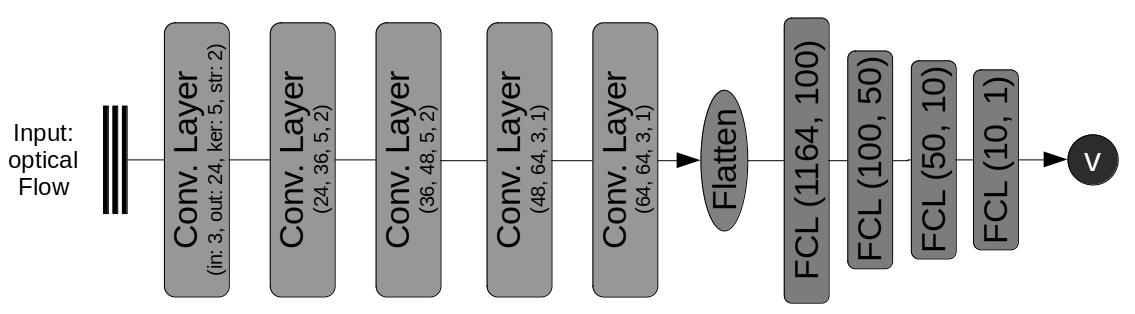
\includegraphics[width=0.9\columnwidth]{imgs/InitialNetwork.png}
	\caption{Initial Network using a series of convolutional layers. The resulting feature vector is 
	then flattened and mapped into several fully connected layers.}
	\label{fig:initialNetwork}
\end{figure}

Using the initial model on the training data with a hard splitting, we achieved a MSE between 18 and 20 
in the validation set, while having a MSE of less than 3 on the training set. The initial network 
therefore has some clear overfitting problems, which we tried to address with our fine tuning.

\subsection{Siamese Network}
\label{subsec:SiameseNetork}
In order to improve our results, we also tried to extend the optimized initial network (\cref{sec:fineTuning}) 
to a siamese network, which would allow us to use also the original images as training data. Therefore we used shared weights for the convolutional layers, concatenated 
the two resulting feature vectors and mapped them into the fully connected layers as shown in \cref{fig:siameseNetwork}. This method was inspired by the architecture used in
\cite{Wang2017}. 
\begin{figure}[ht]
	\centering
	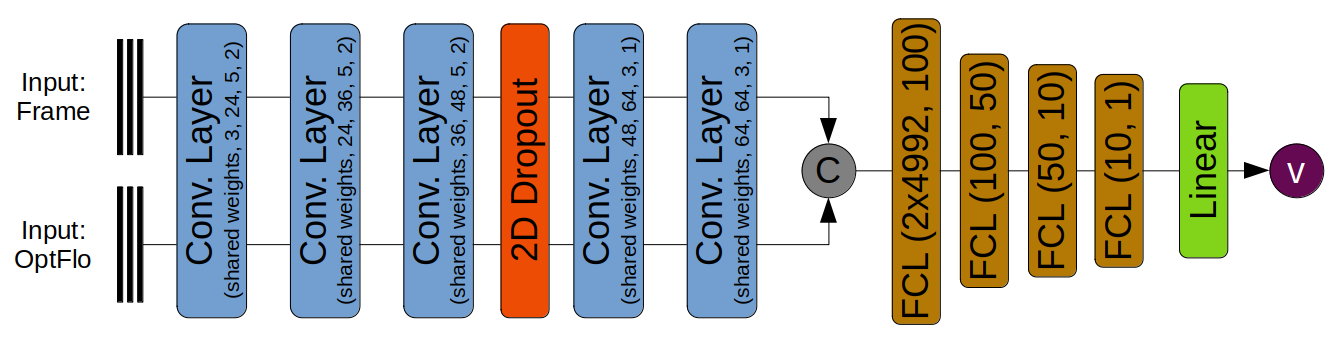
\includegraphics[width=0.9\columnwidth]{imgs/siamese_model.png}
	\caption{Siamese architecture based on the fined tuned original network. The two inputs pass 
	several convolutional layers with shared weights and a drop out layer. The resulting
	feature vectors are concatenated and then mapped into several fully connected layers.}
	\label{fig:siameseNetwork}
\end{figure}
We used this architecture in two different ways: feeding either two consecutive frames into the model, or one image and one optical flow field frame. In order to keep the structure correspondent, we 
sampled down the regarding images to the size of the optical flow field.

\section{Fine tuning}
\label{sec:fineTuning}

We experimented with various different options to fine tune the original model which will be discussed and compared:

\subsection{Batch normalisation and activation functions}
Similar to the lecture, we included batch normalization layers \cite{BatchNorm2015}, to speed up
the training and improve the networks performance.

We also tested different activation functions. As proposed in the lecture, we initially used the ReLu
function
\begin{align*}
\mathrm{ReLu}: \mathbb{R} \to \mathbb{R}_0^+, x \mapsto \max\{0,x\}.
\end{align*}
Using the ReLU function and 15 epochs for training, we achieved a MSE of around 15 on the 
testing set. We ran the code multiple times, to ensure this result holds. This result was not really 
promising, so we wanted to decrease the error by modifying the model even more.

To solve the problem of dead neurons\footnote{One can clearly see in the definition of the ReLU 
function, that neurons with a value below zero cannot participate in the learning process.} of the ReLU function, we 
tried the leakyReLU function
\begin{align*}
\mathrm{leakyReLU} : \mathbb{R} \to \mathbb{R}, x \mapsto \begin{cases}
x, x \geq 0\\
c \cdot x, x <0
\end{cases}
\end{align*}
with a hyperparameter $c{=}0.01$. Using the leakyReLU function, we achieved a MSE of around 12 on the 
testing set and under 3 on the training set. All of the models were trained with only eight epochs, as 
we still had problems with overfitting the data.

\subsection{Dropout Layer}
As we still had a lot of overfitting issues, we decided to include a dropout layer, according to 
\cite{Dropout2014}. We tried different positions and different amounts of dropout layers, but using one 
layer with a probability of $p{=}0.5$ after the third convolutional layer seemed to work best.

\subsection{Pooling layers with initial splitting}
In order to force the network to compress the data even further, we added two generic pooling layers to the network, to reduce the number of parameters\footnote{Indeed, 
the number of parameters decreased from a total of 636.225 trainable parameters to 156.225 --- a 
decrease by a factor of 4. We calculated these numbers using the tool \emph{PyTorch summary} 
(\url{https://github.com/sksq96/pytorch-summary}).} of the model. One after the second 
convolutional layer and the second one right before the fully connected layers start.
We tested maximum and average pooling with the following parameters
\begin{align*}
\text{kernel size} &:= 2\times 2 &\text{\ \ \ \ } \text{stride} &:= 2\\
\text{padding} &:= 1 &\text{\ \ \ }\text{dilatation} &:= \text{None}
\end{align*}
The implementation of pooling layers helped a lot, as now the loss on the train and test data seemed to 
decrease nearly proportionally. Our results with the initial splitting are shown 
\cref{tab:ResultsInitialSplitting}. We also tried the network
with maximum pooling with 15 epochs, as the loss on the train and test set was decreasing in a pretty 
stable manner. Using this network, we achieved for the first time a MSE of under 10 on the test set,
which is, according to our assumptions in \cref{subsec:AimAndMeasure}, a 
pretty good result --- especially, as we trained the model mostly on highway scenes and tested it only 
in city driving scenarios.
\begin{table}[!t]
\normalsize
\centering
\begin{tabular}{lcccc}
\toprule
\multirow{2}{*}{Initial splitting, 8 epochs}  & \multicolumn{2}{c}{$\mathrm{ReLU}$} & \multicolumn{2}{c}{$\mathrm{leakyReLU}$} \\
 & Train & Test & Train & Test\\
\midrule
No pooling & 2.85 & 12.08 & 2.45 & 10.75 \\
Max pooling & 5.62 & 11.82 & 5.52 & 10.29 \\
Max pooling (15 epochs) & - & - & \textbf{3.22} & \textbf{9.63} \\
Average pooling & 7.70 & 11.40 & 6.08 & 13.09\\
\bottomrule
\end{tabular}
\caption{MSE results of the network using different pooling strategies, one dropout layers, two different activation functions and 
the initial splitting. We trained each of the models for eight epochs.}
\label{tab:ResultsInitialSplitting}
\end{table} 

\subsection{Optimizer and scheduler}
For all of our networks we used the \emph{ADAM} \cite{Adam2014} algorithm as a (stochastic) optimizer. 
For scheduling, we tried the \emph{ReduceLROnPlateau}-scheduler of the \emph{PyTorch}\footnote{
\url{https://pytorch.org/docs/stable/index.html}} module and later
switched to the \emph{MultiStepLR}-scheduler.

\section{Error analysis and results}
In order to compare the potential and accuracy of the different predictions we focused on two major points: Firstly comparing the training and validation loss and how they would converge as well as secondly using the velocity-frame chart of the predictions to classify the results as described in \cref{subsec:dataAnalysis}. These results are shown in \cref{fig:resultsSummary}. Finally we also compared the performance on the test video to get an indication how the models would perform on a completely unknown data set (\cref{fig:resultsTestvideo}).

\begin{figure}[ht]
	\centering
	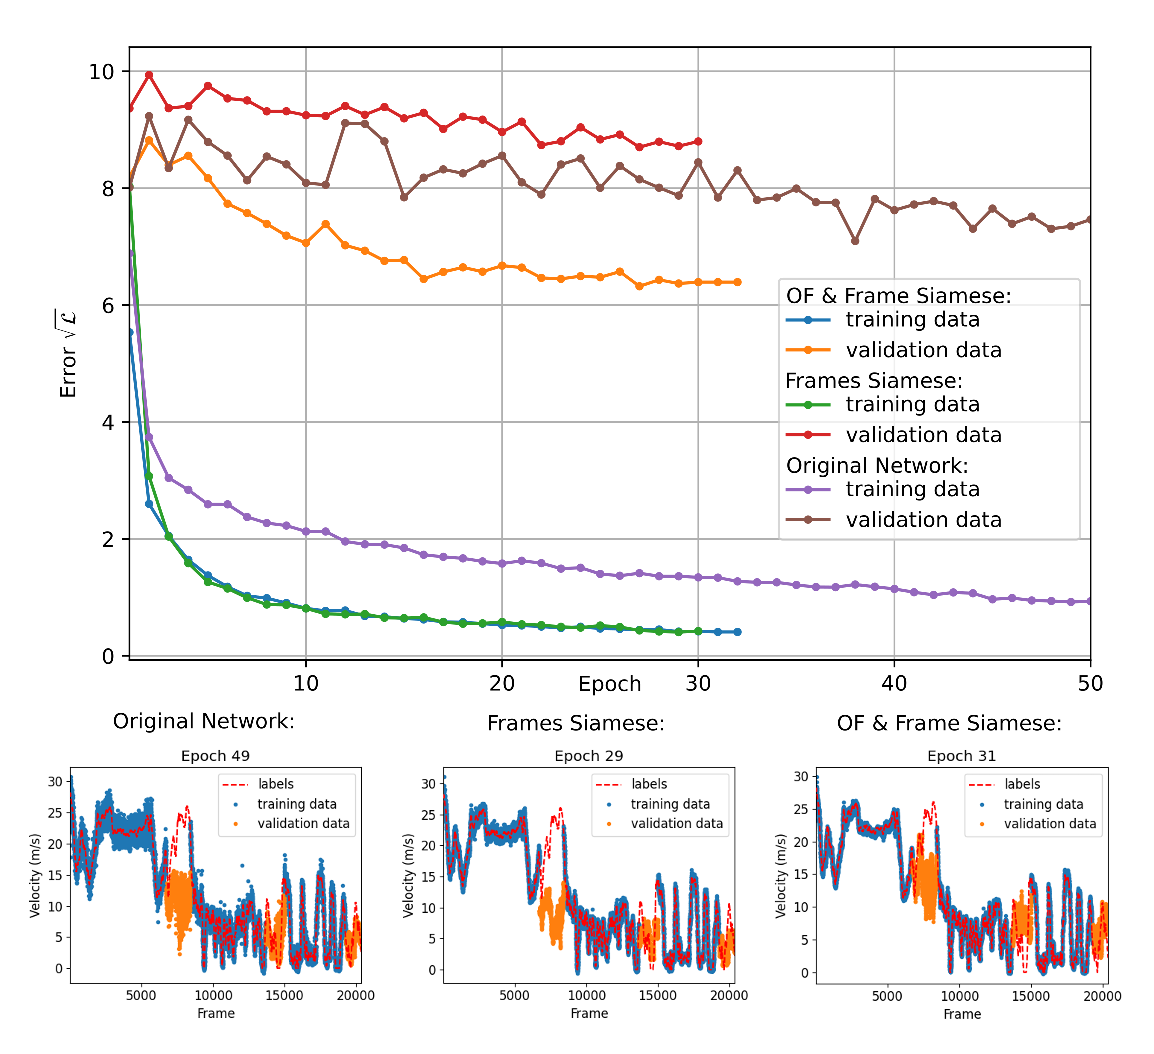
\includegraphics[width=0.99\columnwidth]{imgs/TrainingProcess.eps}
	\caption{Comparison of the results using the models: tuned original network (after 50 epochs: $\sqrt{\mathcal{L}} = 7.46$) and siamese model with frames (after 30 epochs: $\sqrt{\mathcal{L}} = 8.82$) and optical flow (after 50 epochs: $\sqrt{\mathcal{L}} = 6.39$); \textit{top}: training and validation error per epoch; 
	\emph{bottom}: predictions after the last epoch with correct values in red}
	\label{fig:resultsSummary}
\end{figure}

We can identify that the two siamese approaches perform very similarly on the training set while producing only a very raw fitting of the driving scenarios on the validation set. The validation loss of both models converges at about 30 epochs while the training data is almost perfectly fitted. So both models, especially the model using only two frames, still produce a large overfitting. This also results in a very bad performance on the test video, as depicted in \cref{fig:resultsTestvideo}. The model was not even able to decide between different driving scenarios there.

Our optimized original model using only the optical flow showed a better performance. As shown in \ref{fig:resultsSummary} the results did converge much slower but at about the same speed for both training and validation set. We stopped our calculations after 50 epochs but the model did not converge finally yet. We can also determine that the predictions are nearly perfect for city driving and stop and go traffic but only very rough for highway driving. Looking at the predictions on the test set the network was able to distinguish between all three different driving scenarios and did even detect all of the stops during the city driving. Still the absolute velocity may be not entirely correct especially for highway driving.

\begin{figure}[ht]
	\centering
	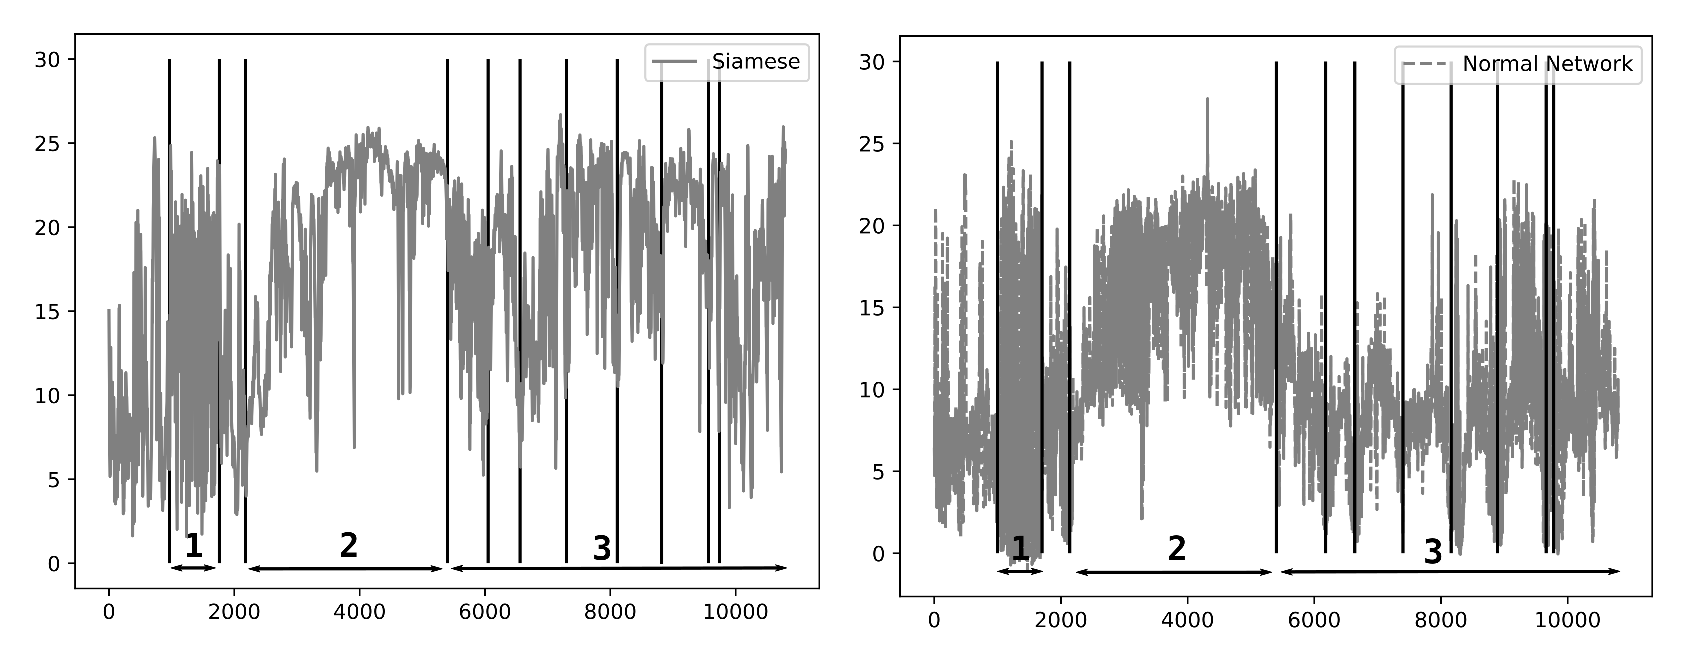
\includegraphics[width=0.99\columnwidth]{imgs/both_testvideo.eps}
	\caption{the networks performance on the test video with the different driving scenarios labeled: 1) longer halt at crossroad, 2) highway driving, 3) city driving with several stops indicated}
	\label{fig:resultsTestvideo}
\end{figure}

\section{Discussion and possible optimizations}

Especially the performance of the optimized original model was very satisfying, considering the small amount of training data. On the other hand, the siamese network did not show the expected 
optimization of the predictions.

Additionally, we identified several problems, that need to be solved, to achieve a better performance:
\begin{enumerate}[label=(\roman*)]
	\item \textbf{Predictions are limited to specific video parameters}, especially to camera perspective and changes in brightness. This issue occurred, when we tried testing our models using our 
	own acquired data. As a solution, rescaling and moving frame cutouts for training, might be a possible approach as well as brightness augmentation.
	\item \textbf{Lack of generalization}: As we also experimented with different splittings of training and validation data, we figured out that using randomly shuffled validation data results in a 
	very good fitting which becomes a qualitative fitting for block splitting and a very rough fitting for different videos. This might be solved by using more data from various different sources.
	\item \textbf{Very complex model trained with very little data}: this issue is rather connected with the second and might as well be solved with a larger data set.
\end{enumerate}


%\subsection{Augmented brightness}
%The calculation of the optical flow field is in general quite sensitive to noise and brightness changes. To make these calculations more robust, we
%tried to add some additional noise to the frames, before calculating the flow field. To change the brightness and contrast of an image, we used
%the formula
%\begin{align*}
%\mathrm{frame}_{\mathrm{augmented}}(i,j) = \alpha(i,j) \cdot \mathrm{frame}(i,j) + \beta(i,j).
%\end{align*}
%The function $\alpha$ controls the contrast augmentation ($>1$ increase, $<1$ decrease) and the function $\beta$ controls the brightness. To 
%get some noise into the frames, we used
%\begin{align*}
%\alpha \sim \mathcal{U}(0,1)+0.35,\; \beta \sim \mathcal{U}(-5,35),
%\end{align*}
%where $\mathcal{U}(a,b)$ denotes the uniform distribution in an interval $[a,b]$ for $a,b\in \mathbb{R}$ with $a < b$. 

%In nearly all of our tests, the upper augmentation process seemed to have only marginal effects on the performance of the networks. We 
%also tried different distribution intervals and also normally distributed functions $\alpha$ and $\beta$, but
%our networks seemed to already be quite invariant to these changes.

\printbibliography

\end{document}
